% ---------------------------------------------------------------------------
% IPT-Model: how the model works
% Beamer deck. Compile with:  pdflatex ipt_model_slides.tex   (run twice)
% Needs only standard packages: beamer, tikz, booktabs, amsmath, lmodern.
% All numbers are taken from the repository (README.md, docs/, and
% data/processed/default/) for the main 2022 configuration.
% ---------------------------------------------------------------------------
\documentclass[aspectratio=169,9pt,t]{beamer}

\usepackage[T1]{fontenc}
\usepackage[utf8]{inputenc}
\usepackage{lmodern}
\usepackage{amsmath,amssymb}
\usepackage{booktabs}
\usepackage{array}
\newcolumntype{L}[1]{>{\raggedright\arraybackslash}p{#1}}
\usepackage{tikz}
\usetikzlibrary{arrows.meta,positioning,calc,fit,backgrounds}

% ----- Look and feel -------------------------------------------------------
\definecolor{ipnavy}{RGB}{20,45,85}
\definecolor{ipblue}{RGB}{40,100,170}
\definecolor{ipred}{RGB}{180,50,45}
\definecolor{ipgreen}{RGB}{35,125,85}
\definecolor{ipgold}{RGB}{190,135,20}
\definecolor{ipgrey}{RGB}{95,100,110}
\definecolor{iplight}{RGB}{236,241,248}

\usetheme{default}
\usefonttheme{professionalfonts}
\setbeamertemplate{navigation symbols}{}
\setbeamercolor{frametitle}{fg=ipnavy}
\setbeamercolor{title}{fg=ipnavy}
\setbeamercolor{structure}{fg=ipblue}
\setbeamercolor{alerted text}{fg=ipred}
\setbeamercolor{block title}{fg=white,bg=ipnavy}
\setbeamercolor{block body}{bg=iplight}
\setbeamercolor{section in toc}{fg=ipnavy}
\setbeamerfont{frametitle}{series=\bfseries,size=\large}
\setbeamerfont{block title}{series=\bfseries,size=\small}
\setbeamertemplate{itemize item}{\color{ipblue}\rule[0.2ex]{0.9ex}{0.9ex}}
\setbeamertemplate{itemize subitem}{\color{ipgrey}--}
\setbeamertemplate{frametitle}{%
  \vspace{0.45em}\insertframetitle\par\vspace{-0.35em}%
  {\color{ipblue}\rule{\textwidth}{0.6pt}}\vspace{0.2em}}
\setbeamertemplate{footline}{%
  \hbox to \paperwidth{\hspace{1em}\color{ipgrey}\tiny
  \insertshorttitle\ \ $\cdot$\ \ \insertsection\hfill
  \insertframenumber\,/\,\inserttotalframenumber\hspace{1em}}\vspace{0.6em}}
\setlength{\leftmargini}{1.2em}
\setlength{\leftmarginii}{1.1em}

\AtBeginSection[]{%
  \begin{frame}[plain,noframenumbering]
    \vfill
    {\color{ipblue}\rule{0.18\textwidth}{2pt}}\par\medskip
    {\usebeamerfont{title}\Large\bfseries\color{ipnavy}\insertsection\par}
    \vfill
  \end{frame}}

% ----- Shortcuts -----------------------------------------------------------
\newcommand{\h}[1]{\hat{#1}}
\newcommand{\key}[1]{\textbf{\color{ipnavy}#1}}
\newcommand{\up}{{\color{ipgreen}$\uparrow$}}
\newcommand{\dn}{{\color{ipred}$\downarrow$}}
\newcommand{\src}[1]{\par\vfill{\tiny\color{ipgrey}#1\par}}
\newcommand{\plain}[1]{{\color{ipgrey}\small\itshape #1}}
\tikzset{
  box/.style={draw=ipnavy,rounded corners=2pt,fill=iplight,align=center,
              inner sep=4pt,font=\small},
  dbox/.style={box,fill=white,draw=ipgrey},
  flow/.style={-{Latex[length=2mm]},thick,draw=ipnavy},
  lab/.style={font=\scriptsize,text=ipgrey,align=center}
}

\title[IPT-Model]{How the IPT-Model Works}
\subtitle{A quantitative general-equilibrium model of interprovincial and
international trade in Canada}
\author{Model walkthrough}
\date{November 2026}

\begin{document}

% ===========================================================================
\begin{frame}[plain,noframenumbering]
  \vspace{2.2em}
  {\color{ipblue}\rule{0.18\textwidth}{2pt}}\par\medskip
  {\Huge\bfseries\color{ipnavy}How the IPT-Model Works\par}
  \medskip
  {\large\color{ipgrey}A quantitative general-equilibrium model of
  interprovincial and international trade in Canada\par}
  \vfill
  {\small Agents, transmission mechanisms, calibration and results\par}
  \smallskip
  {\footnotesize\color{ipgrey}Main configuration: 13 provinces and territories,
  the United States and the rest of the world; 37 sectors; calibrated to 2022\par}
  \vspace{1.5em}
\end{frame}

% ---------------------------------------------------------------------------
\begin{frame}{Roadmap}
  \begin{columns}[T]
    \begin{column}{0.52\textwidth}
      \tableofcontents
    \end{column}
    \begin{column}{0.44\textwidth}
      \begin{block}{How to read this deck}
        \small
        Each technical slide gives the equation the code solves
        \emph{and} a plain-language reading of it
        \plain{(in grey italics, like this)}.\\[0.5em]
        Notation follows the repository: $n$ is the \emph{buyer}
        (importer), $i$ the \emph{seller} (exporter), $j$ and $k$ are sectors.
        A hat means a ratio of new to old: $\h x = x'/x$.
      \end{block}
    \end{column}
  \end{columns}
\end{frame}

% ===========================================================================
\section{The question and the model in brief}
% ===========================================================================

\begin{frame}{What the model is for}
  \begin{columns}[T]
    \begin{column}{0.55\textwidth}
      \textbf{Policy questions}
      \begin{itemize}
        \item How much would real incomes rise if provinces lowered the
              barriers to trading with each other?
        \item Which part of those barriers is policy (regulation, licensing,
              procurement) and which is geography (distance)?
        \item What do US tariffs, and Canadian retaliation, do to each
              province?
        \item Who gains, who loses, and do people move as a result?
      \end{itemize}
      \medskip
      \textbf{Why a general-equilibrium model?}
      \begin{itemize}
        \item A trade cost changes prices, which change sourcing, which
              changes wages, which change prices again.
        \item Industries buy from each other, so a cost cut in one sector
              reaches all the sectors that use its output.
      \end{itemize}
    \end{column}
    \begin{column}{0.41\textwidth}
      \begin{block}{What the model delivers}
        \small
        For any change in trade costs or tariffs, the percentage change,
        relative to 2022, in:
        \begin{itemize}
          \item real income, real income per person and real wages, by region
          \item consumer prices
          \item population (interprovincial migration)
          \item exports, imports and interprovincial trade
          \item output and employment by sector and region
        \end{itemize}
      \end{block}
      \plain{It is a long-run, ``before and after'' comparison of two
      equilibria. It says nothing about the path between them.}
    \end{column}
  \end{columns}
\end{frame}

% ---------------------------------------------------------------------------
\begin{frame}{The model on one slide}
  \begin{columns}[T]
    \begin{column}{0.5\textwidth}
      \textbf{Structure}
      \begin{itemize}
        \item \key{15 regions}: 10 provinces, 3 territories, the United
              States, the rest of the world (ROW).
        \item \key{37 sectors}: 19 goods, 18 services (OECD ICIO industries).
        \item \key{Households} work, earn a wage, spend fixed budget shares
              on the 37 sectors, and choose which province to live in.
        \item \key{Firms} in every sector combine labour with inputs bought
              from all sectors. They differ in productivity and compete on
              price; no firm earns a profit.
        \item \key{Buyers} source each product from the cheapest supplier,
              wherever it is, after paying the trade cost.
        \item \key{Governments} do not optimise. Policy is a set of trade
              costs and tariffs that the user changes.
      \end{itemize}
    \end{column}
    \begin{column}{0.46\textwidth}
      \begin{block}{Chosen by the user (exogenous)}
        \small Trade costs $\tau$, tariffs $t$, trade deficits $D$.
      \end{block}
      \begin{block}{Taken from data, held fixed}
        \small Budget shares $\beta$, input shares $\gamma$, value-added
        shares $\phi$, trade elasticities $\theta$, migration elasticity
        $\kappa$, baseline trade shares $\pi$.
      \end{block}
      \begin{block}{Solved by the model (endogenous)}
        \small Wages $w$, prices $P$, trade shares $\pi'$, spending $X$,
        output $R$, incomes $I$, population $L$.
      \end{block}
    \end{column}
  \end{columns}
\end{frame}

% ---------------------------------------------------------------------------
\begin{frame}{Where the model comes from}
  \small
  \begin{tabular}{@{}L{0.2\textwidth}L{0.75\textwidth}@{}}
    \toprule
    Eaton and Kortum (2002) & Trade arises because producers differ in
      productivity; each buyer picks the cheapest source. Gives a ``gravity''
      equation with one key parameter, the trade elasticity $\theta$.\\
    \addlinespace
    Caliendo and Parro (2015) & Many sectors linked by input-output tables;
      tariffs with revenue; solved in changes from observed data.\\
    \addlinespace
    Albrecht and Tombe (2016) & Applied to Canada's 10 provinces; measures
      internal trade costs and splits them into distance and non-distance
      parts.\\
    \addlinespace
    Alvarez, Krznar and Tombe (2019) & Adds the territories and
      workers who move between provinces.\\
    \addlinespace
    \textbf{IPT-Model} & One configurable code base that nests these
      setups, updated to 2022 data with 37 sectors and the United States as a
      separate region.\\
    \bottomrule
  \end{tabular}

  \bigskip
  \begin{tabular}{@{}lccc@{}}
    \toprule
     & A\&T 2016 & AKT 2019 & \textbf{IPT-Model (main)}\\
    \midrule
    Year & 2010 & 2015 & \textbf{2022}\\
    Regions & 10 prov.\ + ROW & 13 + foreign & \textbf{13 + USA + ROW}\\
    Sectors & 22 & 18 & \textbf{37}\\
    Input-output structure & national & national & \textbf{province-specific}\\
    Trade imbalances & balanced & balanced & \textbf{observed, held fixed}\\
    Labour mobility between provinces & no & yes ($\kappa=1.5$) & \textbf{yes ($\kappa=1.5$)}\\
    \bottomrule
  \end{tabular}
\end{frame}

% ===========================================================================
\section{The agents and how they behave}
% ===========================================================================

\begin{frame}{One region at a glance: who does what}
  \centering
  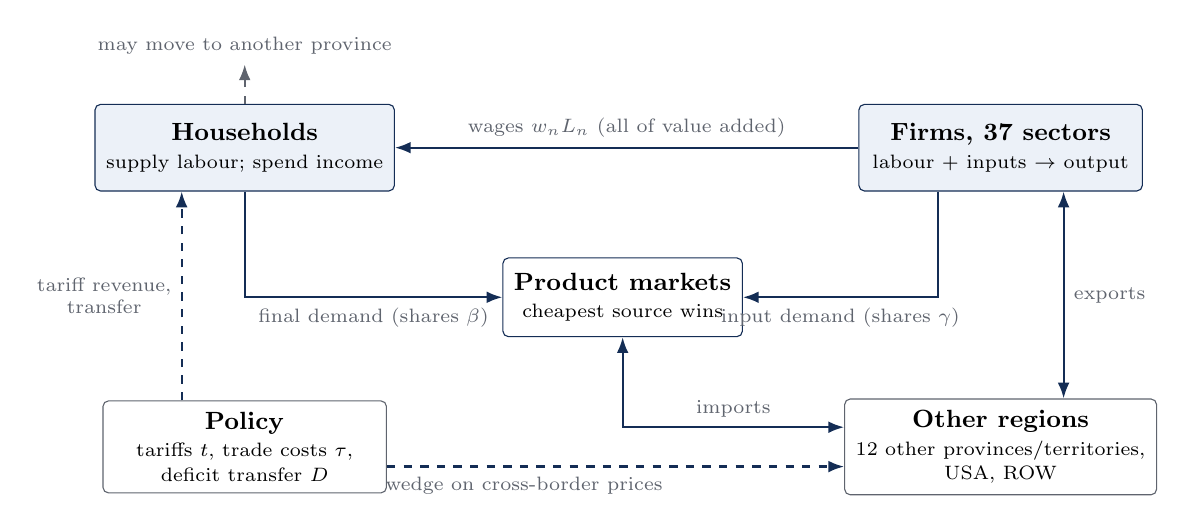
\begin{tikzpicture}
    \node[box,minimum width=3.6cm,minimum height=1.1cm] (hh) at (0,0)
      {\textbf{Households}\\[-1pt]\scriptsize supply labour; spend income};
    \node[box,minimum width=3.6cm,minimum height=1.1cm] (firms) at (9.6,0)
      {\textbf{Firms, 37 sectors}\\[-1pt]\scriptsize labour + inputs $\rightarrow$ output};
    \node[box,fill=white,minimum width=3.0cm,minimum height=1.0cm] (mkt) at (4.8,-1.9)
      {\textbf{Product markets}\\[-1pt]\scriptsize cheapest source wins};
    \node[dbox,minimum width=3.6cm,minimum height=1.1cm] (gov) at (0,-3.8)
      {\textbf{Policy}\\[-1pt]\scriptsize tariffs $t$, trade costs $\tau$,\\[-2pt]\scriptsize deficit transfer $D$};
    \node[dbox,minimum width=3.6cm,minimum height=1.1cm] (row) at (9.6,-3.8)
      {\textbf{Other regions}\\[-1pt]\scriptsize 12 other provinces/territories,\\[-2pt]\scriptsize USA, ROW};

    \draw[flow] (firms.west) -- node[lab,above]{wages $w_nL_n$ (all of value added)} (hh.east);
    \draw[flow] (hh.south) |- node[lab,below,pos=0.75]{final demand (shares $\beta$)} (mkt.west);
    \draw[flow] ([xshift=-8mm]firms.south) |- node[lab,below,pos=0.75]{input demand (shares $\gamma$)} (mkt.east);
    \draw[flow,{Latex[length=2mm]}-{Latex[length=2mm]}] (mkt.south) |- node[lab,above,pos=0.75]{imports} ([yshift=2.5mm]row.west);
    \draw[flow,{Latex[length=2mm]}-{Latex[length=2mm]}] ([xshift=8mm]firms.south) -- node[lab,right]{exports} ([xshift=8mm]row.north);
    \draw[flow,dashed] ([xshift=-8mm]gov.north) -- node[lab,left]{tariff revenue,\\transfer} ([xshift=-8mm]hh.south);
    \draw[flow,dashed] ([yshift=-2.5mm]gov.east) -- node[lab,below,pos=0.3]{wedge on cross-border prices} ([yshift=-2.5mm]row.west);
    \draw[flow,dashed,ipgrey] (hh.north) -- ++(0,0.5) node[lab,above]{may move to another province};
  \end{tikzpicture}

  \medskip
  \plain{Money flows in a closed loop: firms' sales pay for labour and
  inputs; labour income (plus any tariff revenue and transfer) is spent on
  goods and services from every region.}
\end{frame}

% ---------------------------------------------------------------------------
\begin{frame}{Households (1): what they buy}
  \begin{columns}[T]
    \begin{column}{0.53\textwidth}
      \textbf{Preferences.} A resident of region $n$ consumes a bundle from
      each of the $J=37$ sectors:
      \[ U_n=\prod_{j=1}^{J}\big(C_{nj}\big)^{\beta_{nj}},\qquad \sum_j\beta_{nj}=1 . \]
      \plain{Cobb-Douglas: a fixed fraction $\beta_{nj}$ of the budget
      goes to each sector, whatever the prices. If food gets 10\% cheaper,
      the household buys 10\% more of it.}

      \medskip
      \textbf{Within a sector}, each product is bought from the cheapest
      supplier in any region (see firms).

      \textbf{Cost of living.} The price index of region $n$ changes by
      \[ \h P_n=\prod_{j}\h P_{nj}^{\,\beta_{nj}} \]
      \plain{an average of sector price changes, weighted by budget shares.}
    \end{column}
    \begin{column}{0.43\textwidth}
      \begin{block}{Income and welfare}
        \small
        Income of region $n$:
        \[ I_n=\underbrace{w_nL_n}_{\text{labour income}}+\underbrace{D_n}_{\text{deficit}}+\underbrace{T_n}_{\text{tariff revenue}} \]
        Welfare is \key{real income}: $I_n/P_n$.\\[0.4em]
        Change in real income per person:
        \[ \h U_n=\frac{\h I_n}{\h L_n\,\h P_n} \]
      \end{block}
      \small
      \textbf{What ``household'' means here.} $\beta$ is measured on
      \emph{all} final demand in the supply-use tables: household and
      government consumption, non-profits, investment and inventories. One
      representative spender per region stands for all of them.

      \smallskip
      Labour is supplied inelastically: no unemployment, no hours choice.
    \end{column}
  \end{columns}
\end{frame}

% ---------------------------------------------------------------------------
\begin{frame}{Firms (1): technology and costs}
  \begin{columns}[T]
    \begin{column}{0.54\textwidth}
      \textbf{Production.} A producer of product $\nu$ in sector $j$,
      region $i$, with productivity $z$:
      \[ y_{ij}(\nu)=z_{ij}(\nu)\;\ell^{\,\phi_{ij}}\;\Big[\prod_{k=1}^{J} q_k^{\,\gamma_{ikj}}\Big]^{1-\phi_{ij}} \]
      \begin{itemize}
        \item $\phi_{ij}$: share of value added (labour) in gross output.
        \item $\gamma_{ikj}$: share of sector $k$ in sector $j$'s input bill.
        \item Constant returns, perfect competition: price equals cost,
              profits are zero.
      \end{itemize}
      \textbf{Cost of one ``input bundle''} (labour plus materials):
      \[ c_{ij}\;\propto\; w_i^{\,\phi_{ij}}\;\prod_k P_{ik}^{\,(1-\phi_{ij})\gamma_{ikj}} \]
      \plain{An average of the local wage and local input prices. Cheaper
      imported inputs lower the cost of producing locally.}
    \end{column}
    \begin{column}{0.42\textwidth}
      \begin{block}{How firms respond}
        \small
        \begin{itemize}
          \item They spend fixed \emph{shares} of revenue on labour and on
                each input (Cobb-Douglas), so when an input gets cheaper
                they use more of it.
          \item They hire from one regional labour market: the wage is
                the same in every sector of a region, and workers switch
                sector at no cost.
          \item They sell wherever they are the cheapest delivered source.
        \end{itemize}
      \end{block}
      \small
      \textbf{``Labour'' is all of value added.} There is no separate
      capital, land or resource rent. $w_nL_n$ is the region's GDP, and
      the ``wage'' is the return to a composite local factor.

      \smallskip
      $\phi$ and $\gamma$ differ by province, so Alberta's and Ontario's
      industries have different recipes.
    \end{column}
  \end{columns}
\end{frame}

% ---------------------------------------------------------------------------
\begin{frame}{Firms (2): productivity differences and who supplies whom}
  \begin{columns}[T]
    \begin{column}{0.52\textwidth}
      \textbf{Why regions trade.} Each sector has a continuum of products.
      For every product, each region draws a productivity $z$ at random
      (Fr\'echet distribution):
      \begin{itemize}
        \item a region's \emph{average} draw is its overall technology
              $\lambda_{ij}$ (absolute advantage);
        \item the \emph{spread} of draws is governed by $\theta_j$
              (comparative advantage).
      \end{itemize}

      \textbf{Sourcing rule.} The buyer in $n$ compares, product by
      product, the delivered cost from every region $i$,
      \[ \text{delivered cost}=\frac{\kappa_{nij}\,c_{ij}}{z_{ij}(\nu)},\qquad
         \kappa_{nij}=\tau_{nij}(1+t_{nij}), \]
      and buys from the cheapest.

      \medskip
      \plain{Ontario is not best at every kind of machinery. For some
      products Quebec's best producer beats Ontario's even after shipping.
      Lower shipping costs widen the set of products where that happens.}
    \end{column}
    \begin{column}{0.44\textwidth}
      \centering
      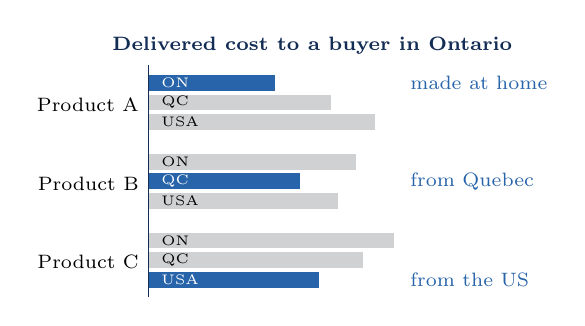
\begin{tikzpicture}[x=0.8cm,y=0.5cm]
        \node[font=\scriptsize\bfseries,text=ipnavy] at (2.6,6.9)
          {Delivered cost to a buyer in Ontario};
        \foreach \y/\name in {5.4/Product A,3.4/Product B,1.4/Product C}
          \node[font=\scriptsize,anchor=east] at (0,\y) {\name};
        % A: ON wins
        \fill[ipblue] (0,5.75) rectangle (2.0,6.15);
        \fill[ipgrey!30] (0,5.25) rectangle (2.9,5.65);
        \fill[ipgrey!30] (0,4.75) rectangle (3.6,5.15);
        % B: QC wins
        \fill[ipgrey!30] (0,3.75) rectangle (3.3,4.15);
        \fill[ipblue] (0,3.25) rectangle (2.4,3.65);
        \fill[ipgrey!30] (0,2.75) rectangle (3.0,3.15);
        % C: USA wins
        \fill[ipgrey!30] (0,1.75) rectangle (3.9,2.15);
        \fill[ipgrey!30] (0,1.25) rectangle (3.4,1.65);
        \fill[ipblue] (0,0.75) rectangle (2.7,1.15);
        \foreach \y/\l/\c in {5.95/ON/white,5.45/QC/black,4.95/USA/black,3.95/ON/black,3.45/QC/white,2.95/USA/black,1.95/ON/black,1.45/QC/black,0.95/USA/white}
          \node[font=\tiny,anchor=west,text=\c] at (0.05,\y) {\l};
        \draw[ipnavy] (0,0.5) -- (0,6.4);
        \node[font=\scriptsize,text=ipblue,anchor=west] at (4.0,5.95) {made at home};
        \node[font=\scriptsize,text=ipblue,anchor=west] at (4.0,3.45) {from Quebec};
        \node[font=\scriptsize,text=ipblue,anchor=west] at (4.0,0.95) {from the US};
      \end{tikzpicture}

      \smallskip
      \begin{block}{Gains from trade, in one sentence}
        \small Each region stops making the products it is relatively bad
        at and buys them from someone better. Average productivity of what
        is still made at home rises.
      \end{block}
    \end{column}
  \end{columns}
\end{frame}

% ---------------------------------------------------------------------------
\begin{frame}{The result of that sourcing rule: a gravity equation}
  Adding up over products gives the share of region $n$'s spending on
  sector $j$ that goes to suppliers in region $i$:
  \[
    \pi_{nij}=\frac{\lambda_{ij}\,(\kappa_{nij}\,c_{ij})^{-\theta_j}}
                   {\sum_{m}\lambda_{mj}\,(\kappa_{nmj}\,c_{mj})^{-\theta_j}}
    \qquad\qquad
    P_{nj}\;\propto\;\Big[\sum_i \lambda_{ij}(\kappa_{nij}c_{ij})^{-\theta_j}\Big]^{-1/\theta_j}
  \]
  \begin{columns}[T]
    \begin{column}{0.5\textwidth}
      \textbf{Reading the trade share}
      \begin{itemize}
        \item Numerator: how competitive $i$ is in $n$'s market: good
              technology ($\lambda$ \up), low costs ($c$ \dn), low barriers
              ($\kappa$ \dn).
        \item Denominator: the same thing for all competitors, including
              $n$ itself. Market shares sum to one.
        \item $\pi_{nnj}$ is the \key{home share}: how much $n$ buys from
              its own producers. It is the model's summary of how closed
              a market is.
      \end{itemize}
    \end{column}
    \begin{column}{0.46\textwidth}
      \textbf{Reading the price index}
      \begin{itemize}
        \item $P_{nj}$ falls when \emph{any} supplier becomes cheaper to
              buy from, in proportion to that supplier's market share.
        \item A region with access to many low-cost suppliers has a low
              cost of living.
      \end{itemize}
      \begin{block}{The elasticity}
        \small A 1\% rise in the cost of buying from $i$ lowers $i$'s sales
        relative to a competitor's by $\theta_j$\%.
      \end{block}
    \end{column}
  \end{columns}
\end{frame}

% ---------------------------------------------------------------------------
\begin{frame}{The trade elasticity $\theta$: the most important parameter}
  \begin{columns}[T]
    \begin{column}{0.5\textwidth}
      \textbf{Two roles, pulling in opposite directions}
      \begin{enumerate}
        \item \textbf{Trade response.} High $\theta$: producers in
              different regions are close substitutes, so a small cost
              change moves a lot of trade.
        \item \textbf{Value of trade.} High $\theta$: little is lost by
              buying at home instead, so each dollar of trade is worth
              less in welfare terms.
      \end{enumerate}
      \plain{Refined petroleum from New Brunswick and from Quebec are
      nearly the same product (high $\theta$). Cars or food products
      differ much more across suppliers (low $\theta$).}

      \medskip
      \textbf{Where the values come from.} Bank of Canada estimates
      (Charbonneau and Landry, 2018) by sector, plus 2 so that the average
      is about 10. The 2016 estimate is used when statistically significant
      ($|t|\ge1.96$), otherwise the 1993 estimate. Services: $5+2=7$.
    \end{column}
    \begin{column}{0.46\textwidth}
      \centering\small
      \begin{tabular}{@{}lr@{}}
        \toprule
        Sector & $\theta_j$\\
        \midrule
        Motor vehicles & 3.0\\
        Agriculture & 3.1\\
        Food, beverages, tobacco & 3.5\\
        Chemicals and pharmaceuticals & 6.8\\
        All 18 service sectors & 7.0\\
        Basic metals & 8.2\\
        Machinery and equipment & 15.0\\
        Wood products & 17.8\\
        Oil and gas extraction & 20.2\\
        Metal ores & 45.0\\
        Refined petroleum & 71.1\\
        \bottomrule
      \end{tabular}

      \medskip
      \raggedright\footnotesize
      \alert{Caution.} The very high values make trade in energy and ores
      react almost one-for-all to small cost changes. Results are also
      reported with the elasticities of Albrecht and Tombe (2016) as a
      sensitivity check.
    \end{column}
  \end{columns}
\end{frame}

% ---------------------------------------------------------------------------
\begin{frame}{Trade costs: what stands between a seller and a buyer}
  \begin{columns}[T]
    \begin{column}{0.52\textwidth}
      \textbf{Iceberg costs} $\tau_{nij}\ge 1$\\
      To deliver one unit from $i$ to $n$, a seller must ship
      $\tau_{nij}$ units; the rest ``melts'' on the way.
      \begin{itemize}
        \item $\tau=1.25$ is a 25\% tariff-equivalent barrier.
        \item A catch-all for everything that makes a sale in another
              region costlier than a sale at home: freight, time,
              differing standards and licensing, procurement rules,
              information and marketing costs.
        \item The lost resources are a pure waste: nobody collects them.
        \item Specific to each importer, exporter and sector; need not be
              the same in both directions.
      \end{itemize}
    \end{column}
    \begin{column}{0.44\textwidth}
      \textbf{Tariffs} $t_{nij}$\\
      An ad valorem tax charged by $n$ on imports from $i$.
      \begin{itemize}
        \item Raises the buyer's price just like an iceberg cost:
              $\kappa_{nij}=\tau_{nij}(1+t_{nij})$.
        \item But the money is collected and returned to the importing
              region's residents.
      \end{itemize}
      \begin{block}{Why the distinction matters}
        \small Removing an iceberg cost frees up real resources.
        Removing a tariff mostly redistributes revenue, with a smaller
        efficiency gain. The same percentage change is therefore worth
        more when it is an iceberg cost.
      \end{block}
    \end{column}
  \end{columns}
  \medskip
  \plain{Internal barriers are modelled as iceberg costs: complying with
  another province's rules uses up real resources and raises no revenue.}
\end{frame}

% ---------------------------------------------------------------------------
\begin{frame}{Governments: a policy lever, not a decision-maker}
  \begin{columns}[T]
    \begin{column}{0.5\textwidth}
      \textbf{What governments do in the model}
      \begin{itemize}
        \item \key{Set trade policy.} Tariffs and policy-related trade
              costs are inputs chosen by the user. No government chooses
              them to maximise anything; there is no strategic
              retaliation unless the scenario specifies it.
        \item \key{Rebate tariff revenue.} With the ad valorem treatment,
              revenue
              $T_n=\sum_{i,j}\frac{t_{nij}}{1+t_{nij}}\pi_{nij}X_{nj}$
              is handed back lump-sum to residents of the importing
              region.
        \item \key{Buy goods and services.} Government consumption and
              investment are part of final demand and so of the budget
              shares $\beta$.
      \end{itemize}
    \end{column}
    \begin{column}{0.46\textwidth}
      \textbf{What they do not do}
      \begin{itemize}
        \item No income or sales taxes, no budget constraint, no public
              debt.
        \item No explicit federal transfers (equalization). Net transfers
              and capital flows appear only through the fixed trade
              imbalance $D_n$.
        \item Public administration is a sector like any other.
      \end{itemize}
      \begin{block}{Two ways to model a tariff (a user option)}
        \small
        \texttt{iceberg} (default, legacy): the tariff is added to $\tau$;
        no revenue. An upper bound on the cost.\\[0.3em]
        \texttt{ad\_valorem}: a true tax with revenue rebated, as in
        Caliendo and Parro (2015).
      \end{block}
    \end{column}
  \end{columns}
\end{frame}

% ---------------------------------------------------------------------------
\begin{frame}{Households (2): where they live}
  \begin{columns}[T]
    \begin{column}{0.54\textwidth}
      \textbf{Location choice.} Each worker has a personal taste for each
      province (random, Fr\'echet with dispersion $\kappa$) and lives where
      \emph{real income per person $\times$ personal taste} is highest.

      \medskip
      The share of Canada's population in province $n$ then changes by
      \[ \h L_n=\frac{\h U_n^{\,\kappa}}{\sum_{m\in\mathcal M}\ell_m\,\h U_m^{\,\kappa}},
         \qquad \h U_n=\frac{\h I_n}{\h L_n\h P_n} \]
      where $\ell_m$ are 2022 population shares and $\mathcal M$ the 13
      provinces and territories.

      \medskip
      \plain{If real income per person in Alberta rises 1\% more than the
      Canadian average, Alberta's population rises by about
      $\kappa=1.5$\% in the long run. People with strong attachment to
      their home province stay; those close to indifferent move.}
    \end{column}
    \begin{column}{0.42\textwidth}
      \begin{block}{Properties}
        \small
        \begin{itemize}
          \item Total Canadian population is fixed; no international
                migration. US and ROW populations are fixed.
          \item $\kappa=1.5$ (Alvarez, Krznar and Tombe, 2019).
                $\kappa=0$ switches migration off (Albrecht and Tombe,
                2016).
          \item Only \emph{changes} matter: existing differences in
                amenities and moving costs are absorbed in the baseline.
        \end{itemize}
      \end{block}
      \small
      \textbf{A dampening force.} More residents share the same fixed
      deficit transfer and tariff revenue, and push the local wage down.\\[0.3em]
      \textbf{A missing one.} There is no housing or land, so nothing
      else slows inflows. Large regional population responses should be
      read with that in mind.
    \end{column}
  \end{columns}
\end{frame}

% ---------------------------------------------------------------------------
\begin{frame}{Putting the agents together: equilibrium}
  An equilibrium is a set of wages and prices such that every market
  clears.
  \medskip
  \begin{columns}[T]
    \begin{column}{0.56\textwidth}
      \small
      \textbf{1. Spending} on sector $j$ in region $n$ = input purchases by
      local firms + final demand:
      \[ X_{nj}=\sum_k\gamma_{njk}(1-\phi_{nk})R_{nk}+\beta_{nj}I_n \]
      \textbf{2. Sales} of sector $j$ in region $i$ = what every region
      buys from it, net of tariffs:
      \[ R_{ij}=\sum_n\frac{\pi_{nij}X_{nj}}{1+t_{nij}} \]
      \textbf{3. Labour market}: labour income = value added of all
      local sectors:
      \[ w_nL_n=\sum_j\phi_{nj}R_{nj} \]
      \textbf{4. Budget}: $I_n=w_nL_n+D_n+T_n$, with $\sum_nD_n=0$.
    \end{column}
    \begin{column}{0.4\textwidth}
      \begin{block}{In words}
        \small
        \begin{itemize}
          \item Every dollar a firm earns is paid to workers or to
                suppliers.
          \item Every dollar of income is spent.
          \item The wage in each region adjusts until the labour that
                firms want (given world demand for the region's products)
                equals the labour available.
          \item A region can spend more than it earns only by the fixed
                amount $D_n$.
        \end{itemize}
      \end{block}
      \small
      Nominal values are measured relative to world value added (the
      numeraire), so only relative wages and real variables are
      meaningful.
    \end{column}
  \end{columns}
\end{frame}

% ===========================================================================
\section{Transmission mechanisms}
% ===========================================================================

\begin{frame}{What happens when an interprovincial trade cost falls}
  \centering
  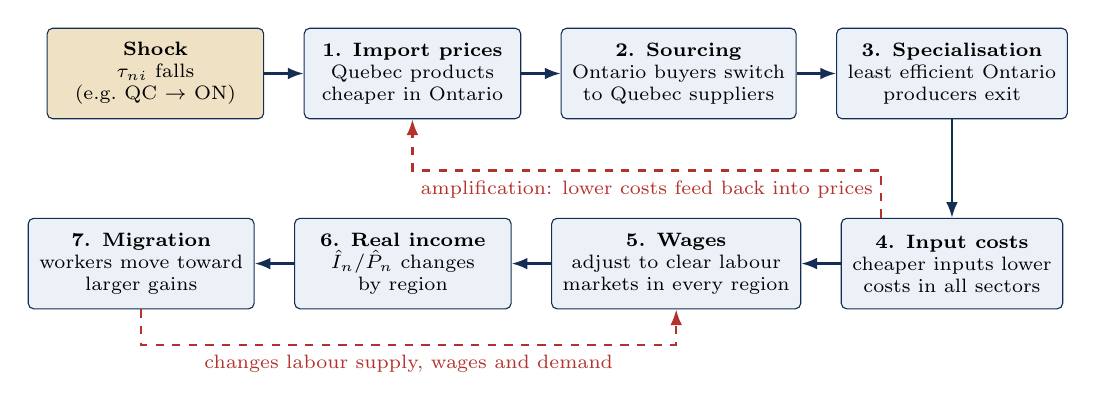
\begin{tikzpicture}[node distance=0.55cm and 0.5cm,
      st/.style={box,minimum width=2.75cm,minimum height=1.15cm,font=\scriptsize}]
    \node[st,fill=ipgold!25] (s0) {\textbf{Shock}\\$\tau_{ni}$ falls\\(e.g.\ QC $\to$ ON)};
    \node[st,right=of s0] (s1) {\textbf{1. Import prices}\\Quebec products\\cheaper in Ontario};
    \node[st,right=of s1] (s2) {\textbf{2. Sourcing}\\Ontario buyers switch\\to Quebec suppliers};
    \node[st,right=of s2] (s3) {\textbf{3. Specialisation}\\least efficient Ontario\\producers exit};
    \node[st,below=1.25cm of s3] (s4) {\textbf{4. Input costs}\\cheaper inputs lower\\costs in all sectors};
    \node[st,left=of s4] (s5) {\textbf{5. Wages}\\adjust to clear labour\\markets in every region};
    \node[st,left=of s5] (s6) {\textbf{6. Real income}\\$\h I_n/\h P_n$ changes\\by region};
    \node[st,left=of s6] (s7) {\textbf{7. Migration}\\workers move toward\\larger gains};
    \draw[flow] (s0) -- (s1);
    \draw[flow] (s1) -- (s2);
    \draw[flow] (s2) -- (s3);
    \draw[flow] (s3) -- (s4);
    \draw[flow] (s4) -- (s5);
    \draw[flow] (s5) -- (s6);
    \draw[flow] (s6) -- (s7);
    \draw[flow,dashed,ipred] ([xshift=-9mm]s4.north) -- ++(0,0.6) -| node[lab,below,text=ipred,pos=0.25]{amplification: lower costs feed back into prices} (s1.south);
    \draw[flow,dashed,ipred] (s7.south) -- ++(0,-0.45) -| node[lab,below,text=ipred,pos=0.25]{changes labour supply, wages and demand} (s5.south);
  \end{tikzpicture}

  \medskip
  \begin{columns}[T]
    \begin{column}{0.47\textwidth}
      \small Steps 1 to 3 are the \key{direct effect}: a market that was
      closed opens, and resources move to better uses.
    \end{column}
    \begin{column}{0.47\textwidth}
      \small Steps 4 to 7 are \key{general-equilibrium feedbacks}. They are
      the reason a full model is needed, and they are solved jointly.
    \end{column}
  \end{columns}
\end{frame}

% ---------------------------------------------------------------------------
\begin{frame}{Channel 1: prices and sourcing}
  \begin{columns}[T]
    \begin{column}{0.54\textwidth}
      \textbf{Prices.} The price of sector $j$ in region $n$ changes by
      \[ \h P_{nj}=\Big[\sum_i\pi_{nij}\,(\h\kappa_{nij}\,\h c_{ij})^{-\theta_j}\Big]^{-1/\theta_j} \]
      \plain{A weighted average of cost changes across suppliers, with
      weights equal to their current market shares. A cost cut on a
      supplier you barely use helps little at first.}

      \medskip
      \textbf{Sourcing.} Market shares move toward suppliers whose
      delivered cost fell relative to the average:
      \[ \pi'_{nij}=\pi_{nij}\Big(\frac{\h\kappa_{nij}\,\h c_{ij}}{\h P_{nj}}\Big)^{-\theta_j} \]
      \plain{With $\theta=7$, a 10\% cost cut on one small supplier raises
      its market share by roughly $0.9^{-7}\approx 2.1$ times.}
    \end{column}
    \begin{column}{0.42\textwidth}
      \begin{block}{Who is affected, and how}
        \small
        \begin{itemize}
          \item \textbf{Buyers in $n$}: lower prices, more variety of
                sources. Gain.
          \item \textbf{Favoured exporter $i$}: more sales, higher labour
                demand. Gain.
          \item \textbf{Producers in $n$}: lose sales on the products
                where they were marginal.
          \item \textbf{Third regions} that sold to $n$: lose market
                share (\emph{trade diversion}).
        \end{itemize}
      \end{block}
      \small The model keeps track of creation and diversion for all
      $15\times15\times37$ flows at once.
    \end{column}
  \end{columns}
\end{frame}

% ---------------------------------------------------------------------------
\begin{frame}{Channel 2: input-output linkages amplify the gains}
  \begin{columns}[T]
    \begin{column}{0.54\textwidth}
      \textbf{The loop.} Costs depend on input prices, and input prices
      depend on costs:
      \[ \h c_{ij}=\h w_i^{\,\phi_{ij}}\prod_k\h P_{ik}^{\,(1-\phi_{ij})\gamma_{ikj}} \]
      \begin{itemize}
        \item Cheaper transport services lower the cost of producing food;
        \item cheaper food lowers the cost of restaurants;
        \item and so on through the whole input-output table (the
              Leontief inverse).
      \end{itemize}
      \textbf{Size.} With one sector, the gain from a given opening is
      multiplied by $1/\phi$. Value added is about half of gross output,
      so linkages roughly \alert{double} the gain:
      \[ \log\frac{\h w_n}{\h P_n}=-\frac{1}{\theta\,\phi}\,\log\h\pi_{nn} \]
    \end{column}
    \begin{column}{0.42\textwidth}
      \begin{block}{A worked example}
        \small
        Ontario's home share falls from 80\% to 78\%
        ($\h\pi_{nn}=0.975$), $\theta=5$.\\[0.4em]
        \begin{tabular}{@{}lr@{}}
          No input linkages ($\phi=1$): & $+0.5\%$\\
          With linkages ($\phi=0.5$): & $+1.0\%$\\
        \end{tabular}\\[0.4em]
        Real wage gain $=0.975^{-1/(\theta\phi)}-1$.
      \end{block}
      \small
      \textbf{Which sectors matter most?} Those that are large in final
      demand \emph{and} widely used as inputs: transport, trade,
      finance, professional services, energy. A barrier in such a
      sector taxes every sector downstream.

      \smallskip
      \plain{This is the ``interconnected industries'' of Albrecht and
      Tombe's title.}
    \end{column}
  \end{columns}
\end{frame}

% ---------------------------------------------------------------------------
\begin{frame}{Channel 3: wages and the terms of trade}
  \begin{columns}[T]
    \begin{column}{0.52\textwidth}
      \textbf{Why wages must move.} After sourcing shifts, some regions
      face more demand for their output and some less. Labour cannot be
      conjured up or left idle, so the wage adjusts:
      \[ \h w_n\h L_n\,VA_n=\sum_j\phi_{nj}R'_{nj} \]
      \begin{itemize}
        \item Region with rising export demand: wage \up. Its exports
              become dearer, which chokes off part of the extra demand.
        \item Region losing sales: wage \dn. It becomes more competitive
              and wins some sales back.
      \end{itemize}
      \plain{The wage plays the role an exchange rate plays between
      countries: it restores balance between what a region sells and
      what it buys.}
    \end{column}
    \begin{column}{0.44\textwidth}
      \begin{block}{Terms of trade}
        \small A region's real income rises when the price of what it
        sells (its wage) rises relative to the price of what it buys.
        Better access to other markets raises the wage; better access to
        other suppliers lowers the price index. Both raise $w/P$.
      \end{block}
      \small
      \textbf{Within a region}, workers move across sectors freely.
      Sector employment changes by $\h R_{nj}/\h w_n$: sectors whose
      sales grow faster than the regional wage expand; the rest
      shrink. No one is unemployed, but the industry mix changes.

      \smallskip
      \textbf{Fixed deficits.} A deficit region keeps receiving the same
      transfer, so part of its income is insulated from wage changes.
    \end{column}
  \end{columns}
\end{frame}

% ---------------------------------------------------------------------------
\begin{frame}{Channel 4: migration spreads the gains across provinces}
  \begin{columns}[T]
    \begin{column}{0.5\textwidth}
      \textbf{Sequence}
      \begin{enumerate}
        \item Liberalisation raises real income per person by different
              amounts in different provinces.
        \item Workers move toward provinces with above-average gains.
        \item Inflows raise labour supply there: the wage and income per
              person fall back; the reverse in provinces losing people.
        \item Migration stops when the remaining gap is offset by
              people's attachment to where they live.
      \end{enumerate}
      \medskip
      \textbf{Net effect}
      \begin{itemize}
        \item Per-person gains are \emph{more equal} across provinces
              than without migration.
        \item Total real income of a province can move much more than
              income per person.
        \item National income rises a little more.
      \end{itemize}
    \end{column}
    \begin{column}{0.46\textwidth}
      \begin{block}{Three welfare measures, reported side by side}
        \small
        \begin{tabular}{@{}ll@{}}
          Real income & $\h I_n/\h P_n$\\[0.2em]
          Real income per person & $\h I_n/(\h L_n\h P_n)$\\[0.2em]
          Real wage & $\h w_n/\h P_n$\\
        \end{tabular}\\[0.5em]
        They coincide only with balanced trade, no tariffs and no
        migration.
      \end{block}
      \small
      \textbf{An extreme case from the main model.} A 10\% cut in external
      trade costs raises New Brunswick's real income by 115\%, but only
      43\% per person: its refining sector ($\theta=71$) expands
      enormously and population grows by half.

      \smallskip
      \plain{A reminder that very high elasticities combined with
      unrestricted mobility can produce near-corner outcomes.}
    \end{column}
  \end{columns}
\end{frame}

% ---------------------------------------------------------------------------
\begin{frame}{A sufficient statistic: the home share tells you the gain}
  \begin{columns}[T]
    \begin{column}{0.55\textwidth}
      With many sectors, the real-wage change in region $n$ can be written
      (Alvarez, Krznar and Tombe, 2019) as
      \[ \underbrace{\log\frac{\h w_n}{\h P_n}}_{\text{real wage}}
         =\sum_j\; g_{nj}\;\times\;\underbrace{\Big(-\frac{\log\h\pi_{nnj}}{\theta_j}\Big)}_{\text{productivity gain in sector } j} \]
      where $g_{nj}$ is sector $j$'s weight in final demand, scaled up by
      its use as an input (elements of $(I-A)^{-1}\beta$).

      \medskip
      \begin{itemize}
        \item \textbf{$\h\pi_{nnj}<1$}: the region buys less from itself,
              so it has dropped its weakest products.
        \item \textbf{Divide by $\theta_j$}: a given fall in the home share
              is worth more where suppliers are less substitutable.
        \item \textbf{Weight by $g_{nj}$}: gains in heavily used sectors
              count more.
      \end{itemize}
    \end{column}
    \begin{column}{0.41\textwidth}
      \begin{block}{Why this is useful}
        \small
        \begin{itemize}
          \item It explains \emph{any} result of the model after the
                fact: look at which home shares moved, in which sectors.
          \item It shows why small, open provinces gain most: their home
                shares have the most room to move.
          \item It is used as a test: in one-sector cases the code must
                reproduce the Arkolakis, Costinot and Rodr\'iguez-Clare
                (2012) formula exactly.
        \end{itemize}
      \end{block}
      \plain{The formula does not replace the model: the change in home
      shares is itself an equilibrium outcome that has to be solved for.}
    \end{column}
  \end{columns}
\end{frame}

% ---------------------------------------------------------------------------
\begin{frame}{The same machinery in reverse: a US tariff on Canadian exports}
  \centering
  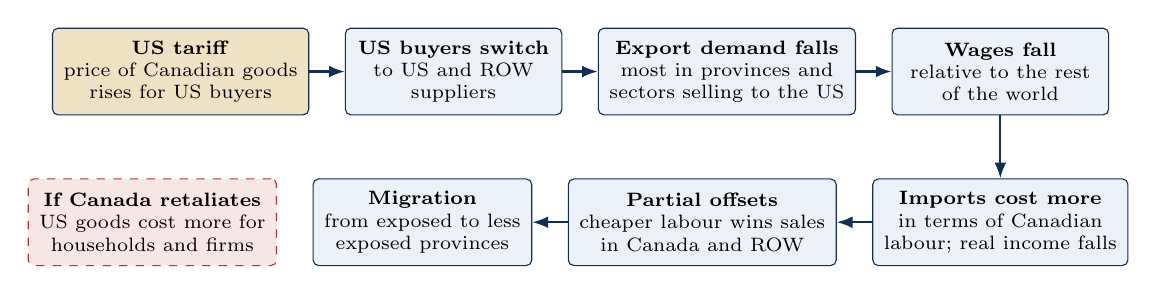
\begin{tikzpicture}[node distance=0.5cm and 0.45cm,
      st/.style={box,minimum width=2.75cm,minimum height=1.1cm,font=\scriptsize}]
    \node[st,fill=ipgold!25] (a) {\textbf{US tariff}\\price of Canadian goods\\rises for US buyers};
    \node[st,right=of a] (b) {\textbf{US buyers switch}\\to US and ROW\\suppliers};
    \node[st,right=of b] (c) {\textbf{Export demand falls}\\most in provinces and\\sectors selling to the US};
    \node[st,right=of c] (d) {\textbf{Wages fall}\\relative to the rest\\of the world};
    \node[st,below=0.8cm of d] (e) {\textbf{Imports cost more}\\in terms of Canadian\\labour; real income falls};
    \node[st,left=of e] (f) {\textbf{Partial offsets}\\cheaper labour wins sales\\in Canada and ROW};
    \node[st,left=of f] (g) {\textbf{Migration}\\from exposed to less\\exposed provinces};
    \node[st,left=of g,fill=ipred!12,draw=ipred,dashed] (h) {\textbf{If Canada retaliates}\\US goods cost more for\\households and firms};
    \draw[flow] (a)--(b); \draw[flow] (b)--(c); \draw[flow] (c)--(d);
    \draw[flow] (d)--(e); \draw[flow] (e)--(f); \draw[flow] (f)--(g);
  \end{tikzpicture}

  \medskip
  \begin{columns}[T]
    \begin{column}{0.47\textwidth}
      \small
      \textbf{Who bears it}
      \begin{itemize}
        \item Canada: worse terms of trade. Its exports fetch less.
        \item US households and firms: higher prices, partly offset by
              tariff revenue if the tariff is modelled as a tax.
        \item ROW: gains some US market share from Canada when only
              Canada is hit; loses when hit too.
      \end{itemize}
    \end{column}
    \begin{column}{0.47\textwidth}
      \small
      \textbf{Retaliation in the model}
      \begin{itemize}
        \item Makes US inputs and consumer goods dearer in Canada, and
              the input-output loop spreads that cost.
        \item Shifts some Canadian demand toward Canadian and ROW
              suppliers, and lowers US wages a little.
        \item On net it lowers Canadian real income further in the
              main results.
      \end{itemize}
    \end{column}
  \end{columns}
\end{frame}

% ---------------------------------------------------------------------------
\begin{frame}{What shapes the regional pattern of results}
  \small
  \begin{tabular}{@{}L{0.27\textwidth}L{0.68\textwidth}@{}}
    \toprule
    Feature of a province & Why it matters\\
    \midrule
    \textbf{Size and openness} & Small provinces buy a larger share of what
      they use from elsewhere. A given cut in trade costs applies to more of
      their spending, so they gain more.\\
    \addlinespace
    \textbf{Trade partners} & Internal liberalisation helps provinces
      oriented to the rest of Canada (Atlantic provinces, territories); a US
      tariff hurts those oriented to the US.\\
    \addlinespace
    \textbf{Sector mix} & Gains are larger where a province trades in
      low-$\theta$ sectors or in sectors with high measured barriers
      (many services).\\
    \addlinespace
    \textbf{Input-output position} & Provinces whose industries rely on
      inputs from other provinces benefit twice: as consumers and as
      producers.\\
    \addlinespace
    \textbf{Size of its barriers} & Measured non-geographic costs differ by
      province: larger for the Atlantic provinces and the territories than
      for Ontario, Alberta and British Columbia.\\
    \addlinespace
    \textbf{Trade imbalance} & Deficit regions (Yukon 41\% of value added,
      Nova Scotia 30\%) fund part of their spending from a fixed transfer,
      so price changes matter more to them than wage changes.\\
    \addlinespace
    \textbf{Migration} & Evens out per-person gains; concentrates
      aggregate gains where people move to.\\
    \bottomrule
  \end{tabular}
\end{frame}

% ===========================================================================
\section{Taking the model to the data}
% ===========================================================================

\begin{frame}{Solving in changes: why so little needs to be estimated}
  \begin{columns}[T]
    \begin{column}{0.53\textwidth}
      \textbf{The problem.} The model in levels has thousands of
      unobservables: technology $\lambda_{ij}$ and trade costs
      $\tau_{nij}$ for every pair and sector.

      \medskip
      \textbf{The trick} (``exact hat algebra'', Dekle, Eaton and Kortum,
      2008). Write every equation as a ratio of the new equilibrium to
      the old. Everything that does not change cancels:
      \[ \frac{\pi'_{nij}}{\pi_{nij}}
         =\Big(\frac{\h\kappa_{nij}\,\h c_{ij}}{\h P_{nj}}\Big)^{-\theta_j} \]
      $\lambda$ has disappeared, and only the \emph{change} in trade
      costs is needed.

      \medskip
      \plain{The observed trade shares already embody all the
      technology and trade-cost differences that produced them. We ask
      only how they would move.}
    \end{column}
    \begin{column}{0.43\textwidth}
      \begin{block}{All that the counterfactual needs}
        \small
        \begin{tabular}{@{}ll@{}}
          $\pi_{nij}$ & trade shares, 2022\\
          $\phi_{nj},\gamma_{nkj}$ & production recipes\\
          $\beta_{nj}$ & final-demand shares\\
          $D_n$ & trade imbalances\\
          $\theta_j$ & trade elasticities\\
          $\kappa$ & migration elasticity\\
          $\h\tau,\,t'$ & the policy experiment\\
        \end{tabular}
      \end{block}
      \small
      \textbf{Not a linear approximation.} The system is solved
      exactly, so it is valid for large shocks (a 35\% tariff,
      eliminating a barrier, even autarky).

      \smallskip
      \textbf{Fit is exact by construction.} With no shock the model
      returns the 2022 data.
    \end{column}
  \end{columns}
\end{frame}

% ---------------------------------------------------------------------------
\begin{frame}{Data}
  \small
  \begin{tabular}{@{}L{0.3\textwidth}L{0.36\textwidth}L{0.28\textwidth}@{}}
    \toprule
    Model object & Source & Notes\\
    \midrule
    Trade among provinces, and each province's purchases from itself
      & Statistics Canada table 12-10-0101-01 (about 500 products)
      & 2010--2022\\
    \addlinespace
    Provincial trade with the US vs.\ ROW
      & Table 12-10-0100-01 (by partner and industry)
      & used to split international flows\\
    \addlinespace
    Trade within and between the US and ROW
      & OECD Inter-Country Input-Output tables, 2025 edition
      & converted to CAD\\
    \addlinespace
    $\phi,\gamma,\beta$ for provinces
      & Provincial supply and use tables (15-602-X)
      & province-specific\\
    \addlinespace
    $\phi,\gamma,\beta$ for US, ROW
      & OECD ICIO & \\
    \addlinespace
    Distances
      & 2021 census: population-weighted centroids of dissemination areas
      & internal distance too\\
    \addlinespace
    Population & Table 17-10-0005-01 & for migration\\
    \addlinespace
    Trade elasticities $\theta_j$
      & Charbonneau and Landry (2018), Bank of Canada
      & alternative: paper values\\
    \bottomrule
  \end{tabular}

  \medskip
  Statistics Canada products and industries are mapped to the 37 sectors by
  classification code, so that Canadian sectors line up with the OECD
  sectors used for the US and ROW.
\end{frame}

% ---------------------------------------------------------------------------
\begin{frame}{Calibration: making the baseline an exact equilibrium}
  \begin{columns}[T]
    \begin{column}{0.53\textwidth}
      \textbf{The issue.} Trade shares, input-output shares and incomes
      come from different sources. Taken together they need not satisfy
      the model's accounting. If they do not, a ``no change'' experiment
      produces changes, and every result is contaminated.

      \medskip
      \textbf{The approach}
      \begin{enumerate}
        \item Take the \emph{shares} $\pi,\phi,\gamma,\beta$ from the data.
        \item Take trade imbalances from the flow matrix:
              $D_n=$ imports $-$ exports (they sum to zero).
        \item \emph{Solve} for the levels of spending, output and value
              added that satisfy market clearing given those shares, with
              world value added equal to the data.
        \item Verify: a shock-free run must return $\h w=\h P=1$ to
              machine precision. The code stops otherwise.
      \end{enumerate}
    \end{column}
    \begin{column}{0.43\textwidth}
      \begin{block}{How close are the solved levels to the data?}
        \small Model value added is within 0.3\% to 6\% of observed value
        added by region in 2022 (largest gaps: Nunavut 6.0\%, Prince
        Edward Island 5.4\%).
      \end{block}
      \small
      \textbf{Trade imbalances are large} and are kept, not assumed away:
      \begin{center}
      \begin{tabular}{@{}lr@{}}
        \toprule
        Region & Deficit, \% of value added\\
        \midrule
        Yukon & $+41$\\
        Nova Scotia & $+30$\\
        New Brunswick & $+22$\\
        Ontario & $+3$\\
        Alberta & $-23$\\
        Saskatchewan & $-23$\\
        \bottomrule
      \end{tabular}
      \end{center}
      Options: hold observed imbalances fixed (default), impose balanced
      trade, or first re-solve the model with zero imbalances.
    \end{column}
  \end{columns}
\end{frame}

% ---------------------------------------------------------------------------
\begin{frame}{Measuring trade costs (1): the Head-Ries index}
  \begin{columns}[T]
    \begin{column}{0.55\textwidth}
      Trade costs are not observed. They are inferred from trade
      itself:
      \[ \bar\tau_{nij}=\left(\frac{\pi_{nnj}\;\pi_{iij}}{\pi_{nij}\;\pi_{inj}}\right)^{\frac{1}{2\theta_j}}
         =\sqrt{\frac{\tau_{nij}\,\tau_{inj}}{\tau_{nnj}\,\tau_{iij}}} \]

      \textbf{Logic}
      \begin{itemize}
        \item If two provinces buy a lot from themselves and little from
              each other, something must be in the way.
        \item Taking the ratio cancels out everything specific to one
              province: its size, its technology, its wages.
        \item $\theta_j$ converts the gap in trade into a cost: with
              highly substitutable products, a small cost explains a
              large gap.
      \end{itemize}
      \plain{$\bar\tau=1.5$ means: shipping between the two provinces
      costs 50\% more than shipping within them, on average over the two
      directions.}
    \end{column}
    \begin{column}{0.41\textwidth}
      \begin{block}{What it is, and is not}
        \small
        \begin{itemize}
          \item A cost \emph{relative to trade within a province}. Costs
                inside a province are not measured.
          \item An average of the two directions.
          \item Everything that reduces cross-border trade, including
                distance and differences in tastes, not only policy.
          \item Sensitive to $\theta_j$: halve the elasticity and the
                cost factor $\bar\tau$ is squared.
        \end{itemize}
      \end{block}
      \small
      \textbf{2022, all interprovincial trade:} average measured cost of
      \alert{56\%} (trade-weighted, 3,254 pair-sector observations).
      Utilities, construction and public administration have no
      estimates and are left unchanged in the experiments.
    \end{column}
  \end{columns}
\end{frame}

% ---------------------------------------------------------------------------
\begin{frame}{Measuring trade costs (2): separating geography from the rest}
  \begin{columns}[T]
    \begin{column}{0.53\textwidth}
      Policy cannot remove distance. For each sector, a regression on
      interprovincial pairs over 2010--2022:
      {\small\[ \log\bar\tau_{nit}=b_1\log\tfrac{d_{ni}}{\sqrt{d_{nn}d_{ii}}}
         +b_2\,\text{adj}_{ni}+\mu_{nt}+\nu_{it}+\varepsilon_{nit} \]}
      \begin{itemize}
        \item $d_{ni}$: distance between provinces, relative to distances
              \emph{within} them; adj$_{ni}$: shared border.
        \item $\mu_{nt},\nu_{it}$: importer-year and exporter-year fixed
              effects.
      \end{itemize}
      \plain{The regression asks: among pairs involving the same
      provinces in the same year, how much higher are costs for pairs
      that are farther apart?}

      \textbf{Decomposition}
      \[ \bar\tau_{ni}=\underbrace{\tau^{geo}_{ni}}_{\text{predicted by distance, adjacency}}
         \times\underbrace{\bar\tau_{ni}/\tau^{geo}_{ni}}_{\text{non-geographic: the rest}} \]
    \end{column}
    \begin{column}{0.43\textwidth}
      \centering
      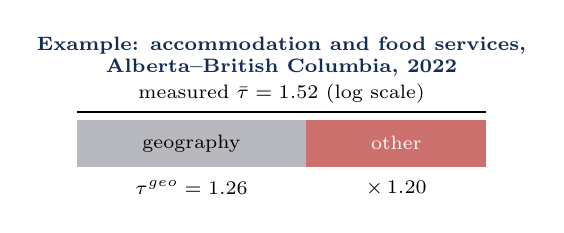
\begin{tikzpicture}[x=5.2cm,y=1cm]
        \node[font=\scriptsize\bfseries,text=ipnavy,align=center] at (0.5,2.0)
          {Example: accommodation and food services,\\Alberta--British Columbia, 2022};
        \fill[ipgrey!45] (0,0.6) rectangle (0.559,1.2);
        \fill[ipred!70] (0.559,0.6) rectangle (1.0,1.2);
        \node[font=\scriptsize] at (0.28,0.9) {geography};
        \node[font=\scriptsize,text=white] at (0.78,0.9) {other};
        \node[font=\scriptsize,anchor=north] at (0.28,0.55) {$\tau^{geo}=1.26$};
        \node[font=\scriptsize,anchor=north] at (0.78,0.55) {$\times\,1.20$};
        \draw[thick] (0,1.3) -- (1.0,1.3);
        \node[font=\scriptsize,anchor=south] at (0.5,1.28) {measured $\bar\tau=1.52$ (log scale)};
      \end{tikzpicture}

      \begin{block}{The experiment this defines}
        \small ``Eliminate non-geographic barriers'':
        \[ \h\tau_{ni}=\min\!\Big(\frac{\max(\tau^{geo}_{ni},1)}{\bar\tau_{ni}},\,1\Big) \]
        In the example, $\h\tau=1.26/1.52=0.83$: a 17\% cut.
      \end{block}
      \raggedright\footnotesize
      \alert{Caveat.} ``Non-geographic'' is a residual. It is an upper
      bound on what policy could remove, not a measure of regulation.
    \end{column}
  \end{columns}
\end{frame}

% ---------------------------------------------------------------------------
\begin{frame}{Measuring trade costs (3): asymmetries}
  \begin{columns}[T]
    \begin{column}{0.53\textwidth}
      The Head-Ries index averages the two directions. But a province may
      find it harder to \emph{export} than to import. Following Waugh
      (2010), let
      \[ \tau_{nij}=\underbrace{t^{s}_{nij}}_{\text{symmetric}}\times\underbrace{t_{ij}}_{\text{exporter-specific}} \]
      The exporter cost $t_{ij}$ is identified from a gravity regression
      of trade shares on distance with importer and exporter effects:
      {\small\[ \log\tfrac{\pi_{nij}}{\pi_{nnj}}=g_j\,x_{ni}+\iota_{nj}+\eta_{ij}+e_{nij},
         \quad \log t_{ij}=-\tfrac{\iota_{ij}+\eta_{ij}}{\theta_j} \]}
      \plain{If a province sells less to everyone than its costs and its
      own purchases would predict, it faces an extra cost of exporting.}

      \medskip
      \textbf{Experiment.} ``Eliminate asymmetries'': lower each cost to
      that of the cheaper direction, $\h\tau_{nij}=\min(1,\,t_{nj}/t_{ij})$.
    \end{column}
    \begin{column}{0.43\textwidth}
      \small
      \textbf{Contribution of asymmetries to export costs, 2022}\\
      (trade-weighted, \%)
      \begin{center}
      \begin{tabular}{@{}lr@{\hspace{1em}}lr@{}}
        \toprule
        Exporter & \% & Exporter & \%\\
        \midrule
        Ontario & 0.7 & Nova Scotia & 19.2\\
        British Columbia & 7.5 & New Brunswick & 23.2\\
        Alberta & 7.5 & Manitoba & 23.8\\
        Quebec & 13.6 & Newfoundland & 36.0\\
         & & P.E.I. & 44.3\\
         & & Saskatchewan & 51.4\\
        \bottomrule
      \end{tabular}
      \end{center}
      \begin{block}{Interpretation}
        \small Smaller and more remote provinces face markedly higher
        costs selling into the large provinces than the reverse.
        Ontario has almost none.
        Average across all trade: about 10\%.
      \end{block}
    \end{column}
  \end{columns}
\end{frame}

% ---------------------------------------------------------------------------
\begin{frame}{What the measured costs look like in 2022}
  \begin{columns}[T]
    \begin{column}{0.56\textwidth}
      \small
      \begin{tabular}{@{}lrrr@{}}
        \toprule
        Trade-weighted, \% & Measured & Geog. & Other\\
         & $\bar\tau-1$ & $\tau^{geo}-1$ & $\frac{\bar\tau}{\tau^{geo}}-1$\\
        \midrule
        \textbf{All sectors} & \textbf{56} & \textbf{60} & \textbf{2}\\
        \midrule
        \emph{Goods}\\
        Agriculture & 202 & 314 & $-16$\\
        Food, beverages, tobacco & 63 & 86 & $-11$\\
        Motor vehicles & 194 & 156 & 18\\
        Computers, electronics & 32 & 5 & 26\\
        Refined petroleum & 4 & 3 & 1\\
        \addlinespace[1pt]
        \emph{Services}\\
        Telecommunications & 80 & 2 & 77\\
        Real estate & 165 & 62 & 68\\
        Education & 134 & 44 & 65\\
        Health and social work & 166 & 65 & 64\\
        Accommodation and food & 74 & 42 & 23\\
        Finance and insurance & 58 & 53 & 4\\
        \bottomrule
      \end{tabular}
    \end{column}
    \begin{column}{0.4\textwidth}
      \textbf{Reading the table}
      \begin{itemize}
        \item Measured costs are large, except in highly substitutable
              commodities.
        \item With distance in logs, geography absorbs most of the
              cost for goods. Negative ``other'': more trade than
              distance predicts.
        \item The non-geographic residual is concentrated in
              \key{services}.
      \end{itemize}
      \begin{block}{Counting only positive residuals}
        \small Setting negative residuals to zero, the average
        non-geographic cost is 9.5\%. This is what the experiment
        removes.
      \end{block}
      {\footnotesize\alert{Specification matters.} With distance in
      kilometres (Alvarez et al., 2019) the same data give about 42\%.}
    \end{column}
  \end{columns}
\end{frame}

% ---------------------------------------------------------------------------
\begin{frame}{From measurement to experiments: the menu of shocks}
  \small
  \begin{tabular}{@{}L{0.27\textwidth}L{0.3\textwidth}L{0.37\textwidth}@{}}
    \toprule
    Scenario type & Change fed to the model & Reading\\
    \midrule
    \texttt{iceberg} & $\h\tau=$ factor & Costs 10\% lower:
      $\h\tau=0.9$\\
    \addlinespace
    \texttt{tariff} (iceberg) & $\h\tau=1+$ rate & Tariff as pure cost, no
      revenue (default)\\
    \addlinespace
    \texttt{tariff} (ad valorem) & $t'=t+$ rate & Tariff as a tax, revenue
      rebated to importer\\
    \addlinespace
    \texttt{measured\_cost\_reduction} & $\h\tau=\dfrac{1+(1-s)(\bar\tau-1)}{\bar\tau}$
      & Cut the measured cost $\bar\tau-1$ by a share $s$\\
    \addlinespace
    \texttt{eliminate\_nongeographic} & $\h\tau=\min\!\big(\max(\tau^{geo},1)/\bar\tau,\,1\big)$
      & Keep only the cost explained by geography\\
    \addlinespace
    \texttt{eliminate\_asymmetries} & $\h\tau=\min(1,\,t_n/t_i)$
      & Bring each cost down to the cheaper direction\\
    \addlinespace
    \texttt{eliminate\_measured} & $\h\tau=\min(1/\bar\tau,\,1)$
      & Trade between provinces as easy as within them\\
    \addlinespace
    \texttt{autarky} & $\h\tau=\infty$ & Shut trade down: the gains from
      existing trade\\
    \bottomrule
  \end{tabular}

  \medskip
  Each shock applies to chosen importers, exporters and sectors, and
  shocks can be combined. A single province recognising other provinces'
  standards is \texttt{eliminate\_nongeographic} with that province as the
  only importer.
\end{frame}

% ===========================================================================
\section{Solving the model}
% ===========================================================================

\begin{frame}{The system that is solved}
  Given baseline data and a shock $(\h\tau,\,t')$, with
  $\h\kappa_{nij}=\h\tau_{nij}(1+t'_{nij})/(1+t_{nij})$, find wage and
  population changes $(\h w_n,\h L_n)$ such that:
  \small
  \begin{columns}[T]
    \begin{column}{0.5\textwidth}
      \begin{align*}
        \text{Costs:}\quad & \h c_{ij}=\h w_i^{\,\phi_{ij}}\textstyle\prod_k\h P_{ik}^{\,(1-\phi_{ij})\gamma_{ikj}}\\[0.3em]
        \text{Prices:}\quad & \h P_{nj}=\Big[\textstyle\sum_i\pi_{nij}(\h\kappa_{nij}\h c_{ij})^{-\theta_j}\Big]^{-1/\theta_j}\\[0.3em]
        \text{Shares:}\quad & \pi'_{nij}=\pi_{nij}\Big(\frac{\h\kappa_{nij}\h c_{ij}}{\h P_{nj}}\Big)^{-\theta_j}\\[0.3em]
        \text{Spending:}\quad & X'_{nj}=\textstyle\sum_k\gamma_{njk}(1-\phi_{nk})R'_{nk}+\beta_{nj}I'_n
      \end{align*}
    \end{column}
    \begin{column}{0.46\textwidth}
      \begin{align*}
        \text{Sales:}\quad & R'_{ij}=\textstyle\sum_n\dfrac{\pi'_{nij}X'_{nj}}{1+t'_{nij}}\\[0.3em]
        \text{Income:}\quad & I'_n=\h w_n\h L_nVA_n+D_n+T'_n\\[0.3em]
        \text{Labour:}\quad & \h w_n\h L_nVA_n=\textstyle\sum_j\phi_{nj}R'_{nj}\\[0.3em]
        \text{Migration:}\quad & \h L_n=\dfrac{\h U_n^{\,\kappa}}{\sum_m\ell_m\h U_m^{\,\kappa}}
      \end{align*}
    \end{column}
  \end{columns}
  \normalsize
  \medskip
  Numeraire: world value added is unchanged, $\sum_n\h w_n\h L_nVA_n=\sum_nVA_n$.

  \medskip
  \plain{Unknowns: 15 wages and 13 populations. Everything else (555 sector
  prices, 8,325 trade shares, spending, sales) follows from them.}
\end{frame}

% ---------------------------------------------------------------------------
\begin{frame}{Solution algorithm: three nested steps}
  \begin{columns}[T]
    \begin{column}{0.5\textwidth}
      \centering
      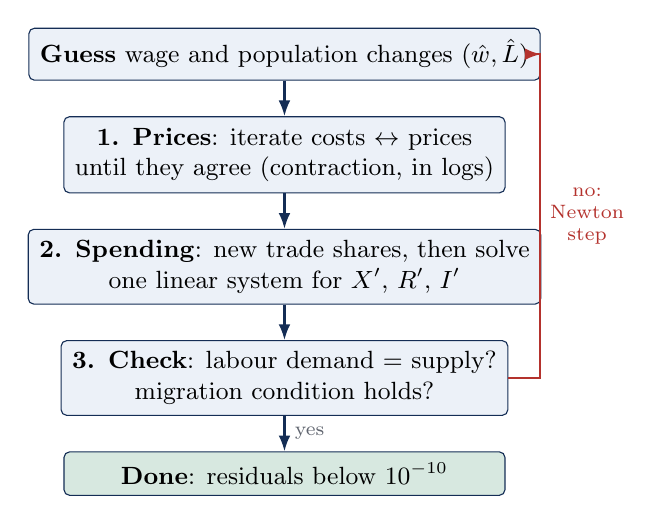
\begin{tikzpicture}[node distance=0.45cm]
        \node[box,minimum width=5.6cm] (g) {\textbf{Guess} wage and population changes $(\h w,\h L)$};
        \node[box,minimum width=5.6cm,below=of g] (p) {\textbf{1. Prices}: iterate costs $\leftrightarrow$ prices\\until they agree (contraction, in logs)};
        \node[box,minimum width=5.6cm,below=of p] (x) {\textbf{2. Spending}: new trade shares, then solve\\one linear system for $X'$, $R'$, $I'$};
        \node[box,minimum width=5.6cm,below=of x] (c) {\textbf{3. Check}: labour demand = supply?\\migration condition holds?};
        \node[box,fill=ipgreen!18,minimum width=5.6cm,below=of c] (d) {\textbf{Done}: residuals below $10^{-10}$};
        \draw[flow] (g)--(p); \draw[flow] (p)--(x); \draw[flow] (x)--(c);
        \draw[flow] (c)-- node[lab,right]{yes} (d);
        \draw[flow,ipred] (c.east) -- ++(0.4,0) |- node[lab,right,pos=0.25,text=ipred]{no:\\Newton\\step} (g.east);
      \end{tikzpicture}
    \end{column}
    \begin{column}{0.46\textwidth}
      \small
      \textbf{Why this ordering works}
      \begin{itemize}
        \item Given wages, prices are a well-behaved fixed point: each
              round of the input-output loop passes on less than 100\%
              of a price change (since $1-\phi<1$).
        \item Given prices and shares, the spending system is linear.
        \item Only the outer problem (28 unknowns) is non-linear. It is
              solved by Newton's method with a line search.
      \end{itemize}
      \textbf{In practice}
      \begin{itemize}
        \item Typical scenario: 3 to 8 Newton steps, 5 to 15 seconds.
        \item Computed in logs so that elasticities as high as 71 do not
              cause numerical overflow.
        \item One market is dropped (Walras' law) and replaced by the
              numeraire.
      \end{itemize}
    \end{column}
  \end{columns}
\end{frame}

% ---------------------------------------------------------------------------
\begin{frame}{How do we know the answers are right?}
  \begin{columns}[T]
    \begin{column}{0.48\textwidth}
      \textbf{Internal checks}
      \begin{itemize}
        \item No shock returns the baseline to machine precision.
        \item Every solution is tested against every equilibrium
              condition.
        \item One-sector cases reproduce the textbook welfare formula
              $\h\pi_{nn}^{-1/(\theta\phi)}$, for small shocks and for
              autarky.
        \item Tariff revenue adds up; population is conserved under
              migration.
        \item On synthetic data, the measurement code recovers the true
              trade costs, exporter costs and gravity coefficients.
        \item \textbf{Independent check:} a separate Python
              implementation with a different solver reproduces the R
              results to about $10^{-13}$.
      \end{itemize}
    \end{column}
    \begin{column}{0.48\textwidth}
      \textbf{Replication of published work}\\[0.3em]
      \small
      \begin{tabular}{@{}L{0.6\textwidth}rr@{}}
        \toprule
        Canada real income, \% & Paper & Here\\
        \midrule
        \multicolumn{3}{@{}l}{\emph{Albrecht and Tombe (2016), 2010 setup}}\\
        Gains from internal trade & 4.4 & 4.5\\
        10\% lower internal costs & 3.6 & 3.4\\
        Eliminate non-distance costs & 6.8 & 7.0\\
        Eliminate all measured costs & 51.9 & 53.1\\
        \addlinespace
        \multicolumn{3}{@{}l}{\emph{Alvarez, Krznar, Tombe (2019), 2015 setup}}\\
        Gains from internal trade & 5.1 & 4.5\\
        Gains from all trade & 19.6 & 18.9\\
        Non-geographic, goods & 3.8 & 5.6\\
        \bottomrule
      \end{tabular}

      \medskip
      \normalsize
      \plain{The solver and data reproduce the 2016 paper closely. The
      2019 gap comes from measured costs, not from the model.}
    \end{column}
  \end{columns}
\end{frame}

% ===========================================================================
\section{Results and how to read them}
% ===========================================================================

\begin{frame}{Internal trade: Canada-wide real income gains (2022 calibration)}
  \begin{columns}[T]
    \begin{column}{0.6\textwidth}
      \small
      \begin{tabular}{@{}L{0.6\textwidth}rr@{}}
        \toprule
        Change in real income, \% & Main & Paper $\theta$\\
        \midrule
        \emph{Uniform cuts}\\
        10\% lower interprovincial costs & 4.0 & 3.2\\
        10\% lower cost of imports from abroad & 3.1 & 2.8\\
        10\% lower costs with abroad, both ways & 9.0 & 6.7\\
        \addlinespace
        \emph{Based on measured costs}\\
        10\% lower measured interprovincial costs & 0.7 & 0.8\\
        Eliminate asymmetries & 4.8 & 5.6\\
        \textbf{Eliminate non-geographic barriers} & \textbf{4.9} & \textbf{6.7}\\
        \quad goods only & 0.5 & 0.6\\
        \quad services only & 4.4 & 6.0\\
        Eliminate all measured costs & 46.2 & 61.0\\
        \bottomrule
      \end{tabular}

      \smallskip
      {\tiny\color{ipgrey} Baseline-income weights, labour mobility with
      $\kappa=1.5$. ``Paper $\theta$'': elasticities of Albrecht and Tombe
      (2016). Source: README.md.}
    \end{column}
    \begin{column}{0.36\textwidth}
      \textbf{Reading the numbers}
      \begin{itemize}
        \item A 10\% uniform cut is worth about 4\% of real income: more
              than the direct saving, because of input-output
              amplification.
        \item Removing non-geographic barriers is worth about 5\%. Nearly
              all of it comes from \key{services}.
        \item Asymmetries are worth about as much again.
        \item ``Eliminate all'' (46\%) is a thought experiment: it
              removes distance too.
      \end{itemize}
      \plain{Published figures for comparison: 6.8\% (A\&T) and 4.4\%
      (Manucha and Tombe, 2022) for non-geographic barriers.}
    \end{column}
  \end{columns}
\end{frame}

% ---------------------------------------------------------------------------
\begin{frame}{US tariffs: Canada-wide real income losses}
  \begin{columns}[T]
    \begin{column}{0.56\textwidth}
      \small
      \begin{tabular}{@{}L{0.72\textwidth}r@{}}
        \toprule
        Change in real income, \% & Main\\
        \midrule
        \emph{Tariff as iceberg cost, all sectors}\\
        US 35\% tariff on all partners & $-3.0$\\
        \quad with Canadian retaliation & $-4.0$\\
        \quad with Canadian and ROW retaliation & $-3.9$\\
        US 50\% tariff on metals & $-0.1$\\
        \quad with Canadian and ROW retaliation & $-0.2$\\
        \addlinespace
        \emph{Tariff as a tax on goods, revenue rebated}\\
        US 35\% tariff & $-2.0$\\
        \quad with Canadian retaliation & $-2.5$\\
        \bottomrule
      \end{tabular}

      \bigskip
      \normalsize
      \centering
      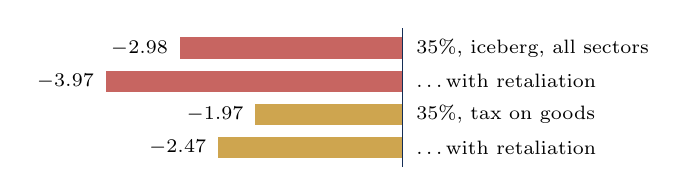
\begin{tikzpicture}[x=0.95cm,y=0.42cm]
        \foreach \y/\v/\l/\c in {3/2.98/{35\%, iceberg, all sectors}/ipred,
                                 2/3.97/{\dots with retaliation}/ipred,
                                 1/1.97/{35\%, tax on goods}/ipgold,
                                 0/2.47/{\dots with retaliation}/ipgold}{
          \fill[\c!75] (0,\y-0.32) rectangle (-\v,\y+0.32);
          \node[font=\scriptsize,anchor=west] at (0.05,\y) {\l};
          \node[font=\scriptsize,anchor=east] at (-\v-0.03,\y) {$-\v$};
        }
        \draw[ipnavy] (0,-0.6) -- (0,3.6);
      \end{tikzpicture}
    \end{column}
    \begin{column}{0.4\textwidth}
      \textbf{Reading the numbers}
      \begin{itemize}
        \item A broad 35\% US tariff costs Canada 2\% to 3\% of real
              income in the long run.
        \item Treatment matters: goods-only, with revenue rebated, gives
              about two-thirds of the iceberg figure.
        \item Retaliation deepens Canada's own loss in both treatments,
              though by less when Canada keeps the revenue.
        \item A sector-specific tariff (metals) is small nationally but
              concentrated in a few provinces and industries.
      \end{itemize}
      \plain{The model has no unemployment, investment response or
      uncertainty. These are long-run reallocation losses only.}
    \end{column}
  \end{columns}
\end{frame}

% ---------------------------------------------------------------------------
\begin{frame}{How robust are the results? Three choices drive the range}
  \small
  \begin{tabular}{@{}L{0.2\textwidth}L{0.42\textwidth}L{0.32\textwidth}@{}}
    \toprule
    Choice & Why it matters & Effect on ``eliminate non-geographic
      barriers''\\
    \midrule
    \textbf{What counts as geography}
      & Distance in logs attributes most of the border effect to
        geography; distance in kilometres attributes it to the residual.
        Interprovincial data alone cannot tell them apart.
      & 4.9\% $\rightarrow$ \alert{25\%} (all sectors)\newline
        0.5\% $\rightarrow$ 5.1\% (goods)\\
    \addlinespace
    \textbf{Trade elasticities}
      & They set both the measured size of barriers and the response to
        removing them.
      & 4.9\% $\rightarrow$ 6.7\% with the papers' values\\
    \addlinespace
    \textbf{Distance measure}
      & Mean distance between residents (vs.\ centroids) makes less of
        the cost geographic.
      & 4.9\% $\rightarrow$ about 6.3\%\\
    \addlinespace
    Labour mobility
      & Adds reallocation gains; mostly changes the regional pattern.
      & modest nationally\\
    \addlinespace
    Imbalances, input-output detail, sector count
      & Each moves national results by less than a tenth.
      & small\\
    \bottomrule
  \end{tabular}

  \smallskip
  \begin{block}{Bottom line}
    The largest uncertainty is not the solver or the data. It is which
    share of measured trade costs policy could actually remove.
  \end{block}
\end{frame}

% ---------------------------------------------------------------------------
\begin{frame}{What the model leaves out}
  \begin{columns}[T]
    \begin{column}{0.48\textwidth}
      \textbf{By design}
      \begin{itemize}
        \item \key{Static.} No capital accumulation, no adjustment path,
              no adjustment costs. Results are long-run levels.
        \item \key{Full employment.} Workers displaced in one sector are
              rehired in another at the regional wage.
        \item \key{One factor.} No distinction between labour, capital and
              resource rents; no distributional effects within a region.
        \item \key{Perfect competition.} No markups, firm entry or
              scale economies.
        \item \key{Fixed shares.} Cobb-Douglas demand and technology:
              spending shares across sectors never change.
        \item \key{Passive governments.} No taxes, transfers or
              equalization beyond fixed imbalances.
      \end{itemize}
    \end{column}
    \begin{column}{0.48\textwidth}
      \textbf{Things to keep in mind when using results}
      \begin{itemize}
        \item No congestion (housing, land): population can pour into a
              booming province.
        \item Very high elasticities for refined petroleum (71), ores
              (45) and oil and gas (20) produce near-corner responses to
              uniform cost cuts.
        \item Trade imbalances are fixed transfers and do not adjust.
        \item Measured ``non-geographic'' costs are residuals, not
              catalogued regulations.
        \item The US and ROW are single regions: no US states, no
              distinction among other partners.
      \end{itemize}
      \begin{block}{Likely direction of bias}
        \small Omitted dynamics and scale effects would add to
        long-run gains; adjustment costs and congestion would subtract
        from them.
      \end{block}
    \end{column}
  \end{columns}
\end{frame}

% ---------------------------------------------------------------------------
\begin{frame}{Takeaways}
  \begin{enumerate}
    \setlength{\itemsep}{0.7em}
    \item \textbf{The engine is comparative advantage with frictions.}
          Buyers pick the cheapest source; trade costs keep them buying
          from weaker local producers. Lower costs let each region drop
          what it does worst.
    \item \textbf{Three forces turn a cost cut into a welfare number:} how
          far home shares fall, how substitutable suppliers are
          ($\theta$), and how intensively the sector is used as an input.
    \item \textbf{Agents are simple and transparent.} Households spend
          fixed budget shares and may move province; firms price at cost
          and use fixed input shares; governments are a set of policy
          wedges.
    \item \textbf{The data do most of the work.} Solving in changes from
          an exactly matched 2022 baseline needs only shares and two sets
          of elasticities.
    \item \textbf{Headline results:} removing non-geographic internal
          barriers raises Canada's real income by about 5\%, mostly through
          services; a broad 35\% US tariff lowers it by 2\% to 4\%.
    \item \textbf{The honest range is wide,} and it is governed by how
          measured costs are split between geography and policy.
  \end{enumerate}
\end{frame}

% ===========================================================================
\appendix
\section{Appendix}
% ===========================================================================

\begin{frame}{Notation}
  \small
  \begin{columns}[T]
    \begin{column}{0.48\textwidth}
      \begin{tabular}{@{}lL{0.6\textwidth}@{}}
        \toprule
        $n,\,i$ & destination (importer), origin (exporter); $N=15$\\
        $j,\,k$ & sectors; $J=37$\\
        $\pi_{nij}$ & share of $n$'s spending on sector $j$ bought from $i$\\
        $\phi_{nj}$ & value-added share of gross output\\
        $\gamma_{nkj}$ & share of input $k$ in sector $j$'s input bill\\
        $\beta_{nj}$ & share of sector $j$ in final demand\\
        $\theta_j$ & trade elasticity\\
        $\kappa$ & migration elasticity\\
        $\tau_{nij}$ & iceberg trade cost from $i$ to $n$\\
        $t_{nij}$ & ad valorem tariff of $n$ on imports from $i$\\
        \bottomrule
      \end{tabular}
    \end{column}
    \begin{column}{0.48\textwidth}
      \begin{tabular}{@{}lL{0.6\textwidth}@{}}
        \toprule
        $\kappa_{nij}$ & $\tau_{nij}(1+t_{nij})$, total wedge on the buyer's price\\
        $c_{ij}$ & unit cost of the input bundle\\
        $P_{nj},\,P_n$ & sector price index; consumer price index\\
        $X_{nj}$ & spending of $n$ on sector $j$\\
        $R_{ij}$ & gross output (sales) of sector $j$ in $i$\\
        $VA_n=w_nL_n$ & value added (labour income)\\
        $D_n$ & trade deficit; $\sum_nD_n=0$\\
        $I_n$ & income (final expenditure)\\
        $\bar\tau,\,\tau^{geo}$ & measured (Head-Ries) cost; geographic part\\
        $\h x$ & $x'/x$\\
        \bottomrule
      \end{tabular}
    \end{column}
  \end{columns}
\end{frame}

% ---------------------------------------------------------------------------
\begin{frame}{Regions and sectors of the main configuration}
  \footnotesize
  \textbf{Regions.} Newfoundland and Labrador, Prince Edward Island, Nova
  Scotia, New Brunswick, Quebec, Ontario, Manitoba, Saskatchewan, Alberta,
  British Columbia, Yukon, Northwest Territories, Nunavut; United States;
  rest of the world (all other OECD ICIO economies).

  \medskip
  \begin{columns}[T]
    \begin{column}{0.6\textwidth}
      \textbf{Goods (19)} with $\theta_j$\\[0.2em]
      \begin{tabular}{@{}lr@{\hspace{1.2em}}lr@{}}
        Agriculture, forestry, fishing & 3.1 & Non-metallic minerals & 5.0\\
        Oil and gas extraction & 20.2 & Basic metals & 8.2\\
        Other mining & 45.0 & Fabricated metals & 11.6\\
        Food, beverages, tobacco & 3.5 & Computers, electronics & 11.8\\
        Textiles, clothing & 7.6 & Electrical equipment & 14.3\\
        Wood products & 17.8 & Machinery & 15.0\\
        Paper and printing & 10.7 & Motor vehicles & 3.0\\
        Refined petroleum & 71.1 & Other transport equip. & 10.7\\
        Chemicals, pharma & 6.8 & Other manufacturing & 7.0\\
        Rubber and plastics & 7.0 & & \\
      \end{tabular}
    \end{column}
    \begin{column}{0.36\textwidth}
      \textbf{Services (18)}, all with $\theta_j=7$\\[0.2em]
      Mining support; utilities; construction; wholesale and retail trade;
      transportation; accommodation and food; publishing and broadcasting;
      telecommunications; IT services; finance and insurance; real estate;
      professional services; administrative services; public
      administration; education; health and social work; arts and
      recreation; other services.

      \medskip
      Utilities, construction and public administration are excluded from
      the trade-cost regressions.
    \end{column}
  \end{columns}
\end{frame}

% ---------------------------------------------------------------------------
\begin{frame}{Running and configuring the model}
  \begin{columns}[T]
    \begin{column}{0.5\textwidth}
      \small
      \textbf{Pipeline} (\texttt{scripts/run\_all.R})
      \begin{enumerate}
        \item Download Statistics Canada tables
        \item Build distances
        \item Build bilateral trade flows
        \item Build $\phi,\gamma,\beta$
        \item Estimate and decompose trade costs
        \item Calibrate and verify the baseline
        \item Run scenarios
      \end{enumerate}
      Processed inputs for the main configuration are committed, so steps
      5 to 7 run without downloads.

      \medskip
      \textbf{A scenario is a few lines of YAML}\\[0.2em]
      {\ttfamily\scriptsize
      - id: lower\_barriers\_goods\\
      \ \ shocks:\\
      \ \ \ \ - \{type: iceberg, importers: domestic,\\
      \ \ \ \ \ \ \ exporters: domestic, sectors: goods,\\
      \ \ \ \ \ \ \ factor: 0.85\}}
    \end{column}
    \begin{column}{0.46\textwidth}
      \small
      \textbf{Main switches}\\[0.2em]
      \begin{tabular}{@{}L{0.42\textwidth}L{0.48\textwidth}@{}}
        \toprule
        Option & Values\\
        \midrule
        Calibration year & 2010--2022\\
        Foreign regions & USA + ROW, or ROW\\
        Sector scheme & 37, or an aggregation\\
        Input-output source & regional, national\\
        Trade elasticities & BoC rule, fixed, uniform\\
        Distance measure & centroid, pairwise\\
        Gravity regressors & log or level distance, adjacency, border\\
        Deficits & data, balanced, purge\\
        Migration elasticity & 1.5, or 0\\
        Tariff treatment & iceberg, ad valorem\\
        Canada weights & income, real income, population\\
        \bottomrule
      \end{tabular}
    \end{column}
  \end{columns}
\end{frame}

% ---------------------------------------------------------------------------
\begin{frame}{References}
  \footnotesize
  \begin{itemize}
    \setlength{\itemsep}{0.25em}
    \item Albrecht, L. and T. Tombe (2016). Internal trade, productivity and
      interconnected industries: A quantitative analysis. \emph{Canadian
      Journal of Economics} 49(1): 237--263.
    \item Alvarez, J., I. Krznar and T. Tombe (2019). Internal trade in
      Canada: Case for liberalization. IMF Working Paper 19/158.
    \item Arkolakis, C., A. Costinot and A. Rodr\'iguez-Clare (2012). New
      trade models, same old gains? \emph{American Economic Review} 102(1):
      94--130.
    \item Caliendo, L. and F. Parro (2015). Estimates of the trade and
      welfare effects of NAFTA. \emph{Review of Economic Studies} 82(1): 1--44.
    \item Charbonneau, K. B. and A. Landry (2018). Estimating the impacts of
      tariff changes: Two illustrative scenarios. Bank of Canada Staff
      Analytical Note 2018-29.
    \item Dekle, R., J. Eaton and S. Kortum (2008). Global rebalancing with
      gravity. \emph{IMF Staff Papers} 55(3): 511--540.
    \item Eaton, J. and S. Kortum (2002). Technology, geography, and trade.
      \emph{Econometrica} 70(5): 1741--1779.
    \item Head, K. and J. Ries (2001). Increasing returns versus national
      product differentiation as an explanation for the pattern of US-Canada
      trade. \emph{American Economic Review} 91(4): 858--876.
    \item Manucha, R. and T. Tombe (2022). \emph{Liberalizing internal trade
      through mutual recognition.} Macdonald-Laurier Institute.
    \item Tombe, T. and X. Zhu (2019). Trade, migration, and productivity: A
      quantitative analysis of China. \emph{American Economic Review} 109(5):
      1843--1872.
    \item Waugh, M. E. (2010). International trade and income differences.
      \emph{American Economic Review} 100(5): 2093--2124.
  \end{itemize}
\end{frame}

\end{document}
